\documentclass{report}
\usepackage{graphicx} % Required for inserting images
\usepackage[italian]{babel} %use this package for a thesis written in Italian
\usepackage[utf8]{inputenx}
\usepackage{indentfirst}
\usepackage{microtype}
%\usepackage{chemformula}
\usepackage{mhchem}
\usepackage{setspace}
\usepackage{yfonts,color}
%\usepackage{siunitx}
\usepackage{comment}
%\usepackage{multirow}
%\usepackage{varioref}
%\usepackage[bottom]{footmisc}
\usepackage{wrapfig}
%\usepackage{float}
%\usepackage{type1cm}
\usepackage{lettrine}
\linespread{1.1}
%\usepackage{chngcntr}
\usepackage[nottoc, notlof, notlot]{tocbibind}
%\onehalfspacing
%\counterwithout{footnote}{chapter}
\usepackage{hyperref}
\usepackage[margin=3cm]{geometry}


\usepackage{caption}
\usepackage{subcaption}

\usepackage{booktabs}
\usepackage{tabularx}
\usepackage{adjustbox}
\usepackage{multirow}
\usepackage{listings}
\usepackage{matlab-prettifier}

\lstset{
    language=Matlab,
    style= Matlab-editor,
    basicstyle=\ttfamily\small,
    numbers=left,
    numberstyle=\tiny,
    stepnumber=1,
    numbersep=8pt,
    breaklines=true,
    frame=single,
    showstringspaces=false,
    tabsize=4
}

\hypersetup{
			hyperfootnotes=true,			
			bookmarks=true,			
			colorlinks=true,
			linkcolor=blue,
            linktoc=page,
			anchorcolor=black,
			citecolor=blue,
			urlcolor=blue,
			pdftitle={Tesi Risi},
			pdfauthor={Lorenzo Risi},
			pdfkeywords={thesis, sapienza, roma, university}
 }

\usepackage{lipsum}
\title{Modelli di sistemi biologici \\ Modulo Jlenia Toppi}
\author{Lorenzo Risi}
\date{September 2026}

\begin{document}


\maketitle
\tableofcontents

\chapter{Introduzione alla complessità}
Tutti i sistemi fisiologici sono caratterizzati dalla loro specifica \textbf{complessità}, ogni modello rappresenta un'\textbf{approssimazione} della complessa realtà. Il modello sviluppato deve tenere conto di: 
\begin{itemize}
    \item La complessità intrinseca che è stata semplificata
    \item Disponibilità dei \textbf{dati} necessari per stimare i parametri
\end{itemize}
Quando si guarda un sistema bisogna comprendere la complessità di quest'ultimo e semplificarla attraverso i dati a disposizione.
Quando si ha un sistema complesso ci si concentra su un "situation focus", dal sistema bisogna estrarre le relazioni rilevanti. Queste ultime possono essere utilizzate per spiegare (in modo approssimativo) il sistema, tuttavia non lo descrive completamente: tutti i modelli sono sbagliati ma alcuni sono utili. Conoscere i limiti del modello è essenziale per migliorarlo.

\section{Complessità dell'organismo umano}

%aggiungi foto slides 

L'organismo umano è un sistema multi-input, multi-output controreazionato. Nel modello vengono presi in considerazione disturbi (fisici o mentali) e constraints ??. Nonostante la complessità del modello è comunque semplificato rispetto al sistema reale. La complessità dipende da vari fattori:
\begin{itemize}
    \item Il numero di elementi del sistema 
    \item Interconnessione tra gli elementi
    \item Il comportamento del sistema \textbf{stocastico} e non deterministico
    \item \textbf{Asimmetria} delle relazioni del sistema (per esempio la crescita differenziale delle cellule)
    \item Vincoli non olonomici (le varie parti del sistema assumono indipendenza) 
    \item Processi tempo-varianti
\end{itemize}

I concetti chiave legati alla complessità fisiologica sono feedback.

\subsection{Feedback}
Il feedback è una proprietà fondamentale dei sistemi biologici che permette il controllo e la regolazione, è quindi un ingrediente fondamentale della complessità che caratterizza i sistemi fisiologici. Il feedback è sinonimo di mutua causalità: la variabile X ha un effetto sulla variabile Y e viceversa Y ha un effetto su X. 
\subsubsection{Negative feedback}
Nel feedback negativo un incremento nella variabile X porta ad un incremento della variabile Y e tale incremento nella variabile Y porta un decremento nella variabile X. Questo permette di mantenere variabili nel range basale, come per esempio il metabolismo del glucosio. Dal processo di digestione dei carboidrati produciamo glucosio che viene immesso nella circolazione (aumento di X), il pancreas produce in risposta insulina (aumento di Y) antagonista del glucosio che porta all'assorbimento del glucosio da parte delle cellule (feedback negativo a X). Il meccanismo di feedback negativo crea \textbf{stabilità}.

%immagine ciclo glucosio

\subsubsection{Positive feedback}
Nel feedback positivo un incremento nella variabile X porta ad un incremento della variabile Y e tale incremento nella variabile Y porta ad un ulteriore incremento nella variabile X. Questo meccanismo non è diffuso nei sistemi biologici poichè causa \textbf{instabilità}. Uno dei pochi esempi di feedback positivo sono le contrazioni uterine del parto. La spinta della testa del bambino sulla cervice genera ad una stimolazione neurologica che porta alla secrezione di ossitocina, quest'ultima entra nel flusso sanguigno e porta alla stimolazione delle contrazioni uterine. 

\subsubsection{Feedback intrinseco}
Nelle reazioni chimiche, si parla di feedback intrinseco se il tasso di decremento della concentrazione di A è proporzionale solo alla sua concentrazione; non intervengono quindi fattori esterni. 
\begin{equation}
    \frac{dC_A}{dt}=-kC_A
\end{equation}
Dove $C_A$ è la concentrazione chimica di A e k è la costante di flusso della reazione. 

%foto feedback intrinseco 
\subsubsection{Feedback nei sistemi dinamici}
Quando il sistema di feedback viene a mancare si ha il passaggio dalla condizione di salute alla patologia. Per esempio il diabete è causato dal malfunzionamento del sistema di feedback dell'insulina. Nel diabete di tipo 1 il ramo di andata, non viene prodotta insulina. Nel diabete di tipo 2 non funziona la parte di controreazione, viene prodotta insulina ma non avviene l'assorbimento al livello cellulare. 
%foto insulina

\subsubsection{Altri tipi di feedback}
L'omeostasi è un processo che dipende dal tempo, questo significa che non possiamo avere solo un feedback di tipo proporzionale ma anche di tipo derivativo e integrale. Per esempio se avessi delle variazioni molto veloci (spike) non verrebbe prodotta abbastanza insulina.
Il feedback di tipo \textbf{proporzionale} può dar luogo a ritardi nell'ottenimento dell'effetto della controreazione.
Il feedback di tipo \textbf{derivativo} permette di tenere conto delle variazioni temporali, e della velocità di variazione, dei valori.
In alcuni sistemi compare anche il feedback di tipo \textbf{integrale} che permette di aggiustare il valore a regime della variabile una voltache è stato applicato il feedback. Si applica un feedback proporzionale all'integrale della differenza tra il valore della variabile controllata e il suo valore atteso. 
%diagramma di feedback

\subsection{Controllo}
I pattern di regolazione e controllo che avvengono nei sistemi
fisiologici sono molti e vari e caratterizzano la complessità
dell'organismo umano (interni all'organismo - \textbf{omeostasi}, o
esterni – \textbf{gestione stimoli} in ingresso agli organi di senso). Gli strumenti di controllo per il mantenimento dello stato vitale sono:
\begin{itemize}
    \item Equilibrio statico e dinamico
    \item Regolazione lineare e non lineare
\end{itemize}
Il nostro corpo attua il controllo attraverso due strumenti:
\subsubsection{Enzimi}
Gli enzimi sono catalizzatori biologici delle reazioni chimiche che avvengono nell'organismo umano (aumentano la velocità di reazione):
\begin{equation}
    E+S\longleftrightarrow X \longrightarrow E +P
\end{equation}
Questa è l'equazione di bilancio delle masse dove l'enzima E e il substrato S formano il complesso enzima-substrato XX che a sua volta decompone nell'enzima originale e nel prodotto della reazione P. Il modello del controllo tramite enzimi è complesso e deve essere applicato a tutte le reazioni. 
\begin{figure}[h!]
    \centering
    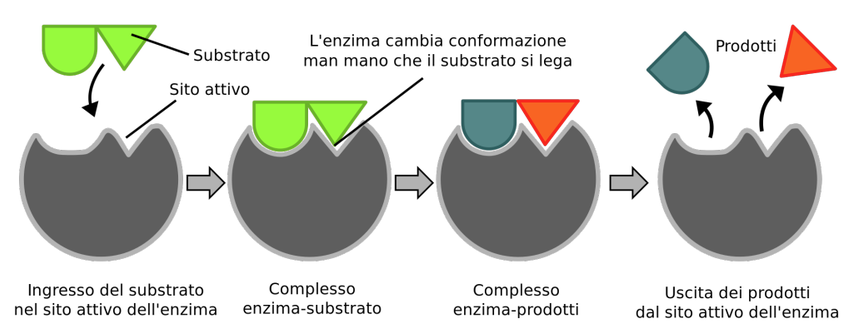
\includegraphics[width=0.75\linewidth]{immagini/enzima.png}
    \caption{Reazione catalizzata da un enzima}
    \label{fig:placeholder}
\end{figure}
\subsubsection{Ormoni}
L'altro processo di controllo avviene attraverso la produzione di ormoni secreti da ghiandole endocrine. Esistono vari tipi di azione ormonale che svolge il nostro corpo: 
\begin{itemize}
    \item \textbf{Azione cinetica}, agisce sulle concentrazioni
    \item \textbf{Azione metabolica}, agisce sui processi metabolici
    \item \textbf{Azione endocrino-cinetica}, 
\end{itemize}
\subsection{Gerarchia}
La struttura dell'organismo umano si
presta ad essere analizzato in termini
di gerarchia: dai geni, alle cellule,
agli organi, fino all'organismo. Ad ogni livello c'è un'azione di feedback e controllo, queste azioni sono coordinate a livello gerarchico e assicurano che gli organi siano in grado di sopportare disturbi normali e anomali sia in termini di grandezza che di scala
temporale.
 
Parte di questo processo è assicurato dalla \textbf{ridondanza}. Per mantenere la funzione in caso di danno ad uno dei due organi o per rendere più sofisticata la funzione. La ridondanza è presente anche nei sistemi di controllo degli organi

\medskip
Per quantificare i processi dinamici e interfacciarsi con la loro complessità è necessario effettuare delle misurazioni, i limiti su cosa può essere misurato sono:
\begin{itemize}
    \item Pratici, dipende dagli strumenti e dai punti di accesso
    \item Etici, dipende dal tipo di misurazione
\end{itemize}
Le misure non devono essere invasive, e per queste si utilizza un approccio diretto e metodi inferenziali.

\chapter{Introduzione alla Modellizzazione}

\begin{wrapfigure}{r}{0.5\textwidth}
  \begin{center}
    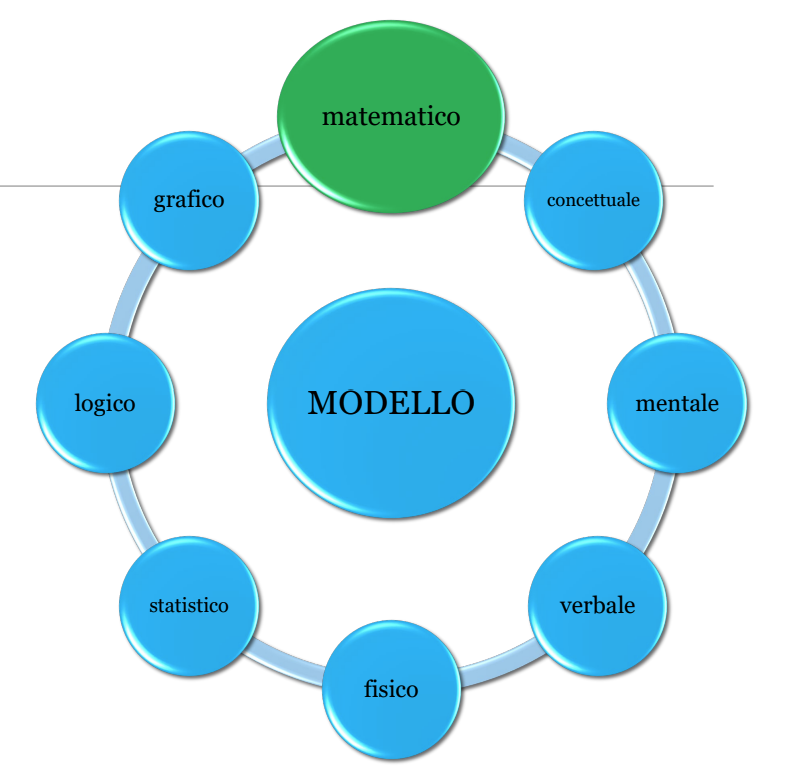
\includegraphics[width=0.5\textwidth]{immagini/tipidimodelli.png}
  \end{center}
\end{wrapfigure}
In ambito biologico e bioingegneristico, un \textbf{modello} può essere definito come una rappresentazione della realtà caratterizzata da un preciso livello di approssimazione. A seconda delle necessità e degli strumenti utilizzati, un modello può assumere diverse forme: può essere concettuale, mentale, verbale, fisico, statistico, logico, grafico o matematico. 

Per comprendere la differenza tra queste tipologie, si consideri l'esempio dell'assorbimento di un farmaco nel sangue. 
\begin{itemize}
    \item \textbf{Modello grafico} rappresenterà visivamente la concentrazione plasmatica del farmaco nel tempo (ad esempio, evidenziando una curva di decadimento esponenziale che descrive un'eliminazione di primo ordine in scala lineare).
    \item \textbf{Modello matematico}, invece, formalizzerà il medesimo processo attraverso un'equazione differenziale, come ad esempio:
\end{itemize}

\medskip
\begin{equation}
\frac{dC}{dt} = -kC
\end{equation}
dove $C$ rappresenta la concentrazione e $k$ la costante di eliminazione.

Il livello di dettaglio di un modello è fondamentale e deve essere sempre bilanciato. Un modello realistico del sistema circolatorio umano, ad esempio, dovrebbe teoricamente descrivere matematicamente il comportamento di ogni singola cellula cardiaca. Tuttavia, un simile livello di dettaglio porterebbe a un sistema di equazioni di dimensioni intrattabili e, di fatto, irrisolvibile. La soluzione risiede nella \textbf{semplificazione}: è possibile scrivere un'equazione per ogni camera cardiaca. Questo introduce un'approssimazione della realtà, ma il livello di dettaglio rimane sufficiente per descrivere correttamente e utilmente il fenomeno macroscopico del pompaggio del sangue.

\section{Obiettivo e Categorie dei Modelli Matematici}

Il modo in cui un modello viene formulato e il livello di dettaglio adottato dipendono principalmente dall'\textbf{obiettivo} del modello stesso. L'obiettivo guida la transizione dal sistema reale alla scelta della metodologia di modellizzazione, fino alla realizzazione del modello finale.
\begin{figure}[h]
    \centering
    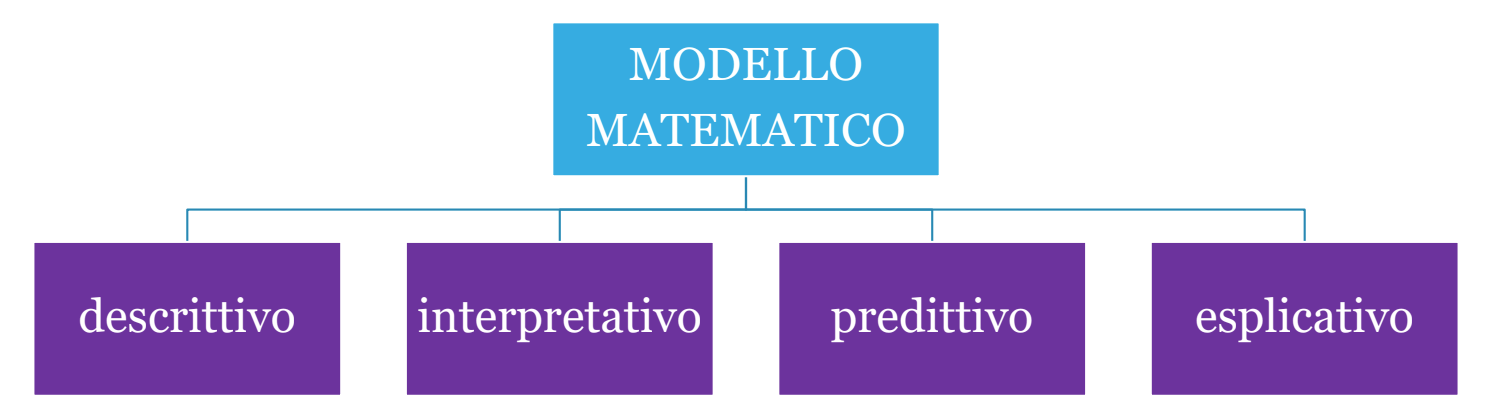
\includegraphics[width=1\linewidth]{immagini/itipidimodello.png}
\end{figure}

\noindent I modelli matematici possono essere suddivisi in quattro categorie principali in base al loro scopo:

\begin{itemize}
    \item \textbf{Descrittivi:} Sono utilizzati per esprimere relazioni quantitative in modo conciso attraverso le equazioni. Questo facilita notevolmente l'analisi e il trattamento dei dati. Ad esempio, se due variabili di un sistema sono direttamente proporzionali, è molto più semplice ed elegante esprimerle tramite un'equazione lineare piuttosto che ricorrere a descrizioni verbali o grafiche.
    \item \textbf{Interpretativi:} Servono a interpretare i dati raccolti o i risultati sperimentali. Riprendendo l'esempio dell'assorbimento di un farmaco nel flusso sanguigno, una curva di decadimento esponenziale rappresenta in modo compatto dei dati che approssimano un processo di primo ordine, permettendo di estrarre parametri utili come la velocità di comparsa (rate of appearance) dall'argomento dell'esponenziale. Permette di spiegare meglio il fenomeno.
    \item \textbf{Predittivi:} Sono impiegati per prevedere come il sistema risponderà a uno stimolo o a un cambiamento interno. Sono lo strumento principe per le \textit{simulazioni}. Ad esempio, conoscendo il modello di un organismo, è possibile simulare l'infusione di un farmaco e valutarne a priori l'effetto terapeutico.
    \item \textbf{Esplicativi:} Hanno l'obiettivo di far comprendere i meccanismi intimi di un fenomeno. In questi modelli, i parametri matematici corrispondono a specifici processi fisiologici; variando tali parametri, è possibile osservare come muta il comportamento globale del sistema, permettendo, ad esempio, la simulazione di comportamenti patologici (come l'attività di neuroni epilettici).
\end{itemize}
Oltre a questi scopi primari, i modelli trovano impiego nella valutazione di ipotesi alternative (confrontando l'accuratezza di vari modelli rispetto a dati reali), nell'inferenza di misure che non possono essere prelevate in vivo, nell'assistenza ai processi educativi (tramite simulatori) e nell'aiuto alla pianificazione sperimentale (ad esempio, definendo gli istanti ottimali per i prelievi di sangue in uno studio di farmacocinetica).
\newpage
\section{Approcci alla Modellizzazione}

Esistono due macro-approcci per modellare un sistema biologico: i modelli basati sui dati e i modelli basati sul sistema fisiologico.

\subsection{Modello dei dati (Data-driven o Black-box)}
Questi modelli forniscono una descrizione quantitativa ricavata puramente dall'analisi dei dati sperimentali di ingresso e uscita (input/output) prelevati dal sistema, senza indagare i meccanismi interni (approccio \textit{black-box}). Esempi tipici sono i sistemi lineari tempo-invarianti (LTI) o le reti neurali artificiali. 
Il modello dei dati dal punto di vista delle procedure di modellizzazione è piu semplice. Il processo di modellizzazione prevede \textbf{due step}: 
\begin{itemize}
    \item Definizione di una rappresentazione input/output del modello: dobbiamo definire le equazioni matematiche (struttura del modello) con cui vogliamo fittare i dati e il grado di complessità del formalismo matematico alla base del modello.
    \item Stima dei parametri: misura dei dati dal sistema sottoponendolo a degli ingressi. Si fa quello che viene chiamato “processo di identificazione” o “stima dei parametri”, sostanzialmente si usano i dati raccolti dal sistema per dare dei valori ai parametri incogniti.
\end{itemize}
Ad esempio possiamo dire che $y=f(u,p)$ dove $y$ è l'uscita, $u$ l'ingresso e $f$ il parametro incognito. Il modello descrittivo, interpretativo e predittivo ricadono all'interno della definizione di modello di dati.
\begin{figure}[h]
    \centering
    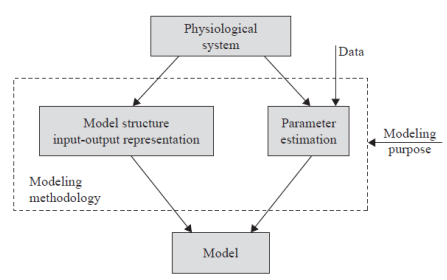
\includegraphics[width=0.5\linewidth]{immagini/modellodatidiagramma.png}
\end{figure}

\subsection{Modello del sistema}
Questo approccio tenta di rappresentare esplicitamente la fisiologia alla base del sistema (ad esempio tramite modelli a compartimenti o circuiti equivalenti). Pur costituendo sempre un'approssimazione della realtà, offre il grande vantaggio di utilizzare variabili e parametri che sono direttamente correlati alle dinamiche e alle proprietà fisiche o biologiche del sistema stesso.
Il processo di formulazione in questo caso è più articolato:
\begin{enumerate}
    \item Formulazione del modello concettuale.
    \item Realizzazione matematica (traduzione in equazioni).
    \item Identificazione a priori dei parametri basata sulle conoscenze fisiche del fenomeno.
    \item Stima o raffinamento dei parametri tramite i dati del sistema.
    \item Soluzione del modello e implementazione computazionale per legare le variabili di interesse.
\end{enumerate}
Il modello esplicativo ricade sicuramente nel modello del sistema; tuttavia, possiamo considerare anche il modello predittivo come modello di sistema (se correlato alle dinamiche fisiche/ biologiche del sistema).
\begin{figure}[h]
    \centering
    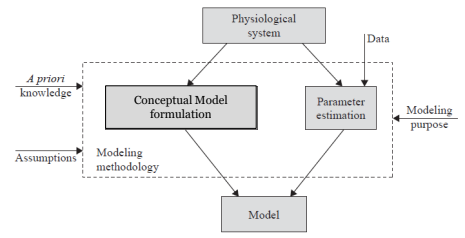
\includegraphics[width=0.55\linewidth]{immagini/modellodelsistema.png}
\end{figure}
\section{L'Approssimazione della Realtà}
Poiché nessun modello può replicare la realtà nella sua interezza, è necessario ricorrere a specifiche tecniche di approssimazione:
\begin{itemize}
    \item \textbf{Aggregazione:} Consiste nell'accorpare parti del sistema reale in macro-elementi. Un esempio classico è la modellizzazione dello spazio extravascolare come un unico grande compartimento, oppure la rappresentazione del rene come singolo blocco anziché modellarne i singoli nefroni.
    \item \textbf{Astrazione:} Prevede di includere nel modello soltanto gli aspetti del sistema che sono pertinenti allo studio. In un modello sulla regolazione del glucosio, ad esempio, si assume che nel circolo sanguigno vi siano solo il glucosio e gli ormoni strettamente correlati ad esso (come l'insulina), ignorando il resto degli elementi ematici.
    \item \textbf{Idealizzazione:} Strutture o comportamenti complessi e difficili da tradurre in formule vengono idealizzati. Ad esempio, si può ipotizzare che un farmaco iniettato si distribuisca istantaneamente e uniformemente in tutto l'organismo, trascurando il transitorio di diffusione.
\end{itemize}
\newpage
\section{Identificazione e Validazione del Modello}
\subsection{Identificazione del modello}

\begin{wrapfigure}{r}{0.5\textwidth}
  \begin{center}
    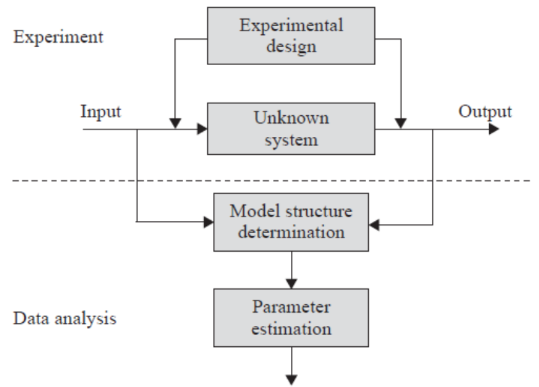
\includegraphics[width=0.5\textwidth]{immagini/indentificazionedelmodello.png}
  \end{center}
\end{wrapfigure}
La transizione dal sistema reale al modello matematico richiede l'esatta definizione della struttura e la determinazione numerica di tutti i suoi parametri. Questo processo, chiamato \textbf{identificazione}, si nutre di dati empirici: confrontando l'uscita misurata con l'uscita del modello si aggiustano i parametri fino a che l'uscita del modello
diviene il più possibile vicina alla misura fatta. I dati possono essere intrinseci al sistema (es. segnali neurali o cardiaci) oppure derivare da esperimenti ad-hoc in cui si applicano stimoli noti (somministrazione di traccianti, variazioni dei gas inspirati) e si misurano le risposte.

\medskip 
\noindent Sorge in questa fase il \textbf{problema dell'identificabilità a priori}: i dati a disposizione sono sufficienti a stimare in modo univoco i parametri del modello? Spesso si assiste a un mismatch tra la complessità del modello scelto e la reale disponibilità di dati. Se il modello possiede troppi parametri rispetto ai dati, occorre semplificarne la struttura (riduzione dell'ordine) oppure arricchire il design sperimentale (acquisendo più campioni o stimolando il sistema in modo diverso). Se invece il modello risulta univocamente identificabile, si procede alla stima formale, tipicamente tramite l'approccio dei minimi quadrati (lineari o non lineari).

\subsection{Validazione}
La validazione ha lo scopo di misurare la bontà del modello rispetto agli obiettivi prefissati e di selezionare il migliore tra modelli alternativi. Si tratta di un processo iterativo: se il modello fallisce i test di validazione, è necessario tornare indietro, modificarne la struttura o le assunzioni, e ripetere l'identificazione.

\noindent I criteri di validazione differiscono dai metodi di stima e includono:
\begin{itemize}
    \item \textbf{Analisi dei residui:} Valutazione quantitativa dell'errore (mismatch) tra l'uscita prodotta dal modello e i dati empirici.
    \item \textbf{Plausibilità fisiologica:} Verifica che i parametri stimati (se il modello è di tipo esplicativo/fisiologico) ricadano in range biologicamente o fisicamente sensati.
    \item \textbf{Parsimonia:} A parità di accuratezza predittiva, va sempre scelto il modello con il minor numero di parametri.
\end{itemize}
\begin{figure}[h]
    \centering
    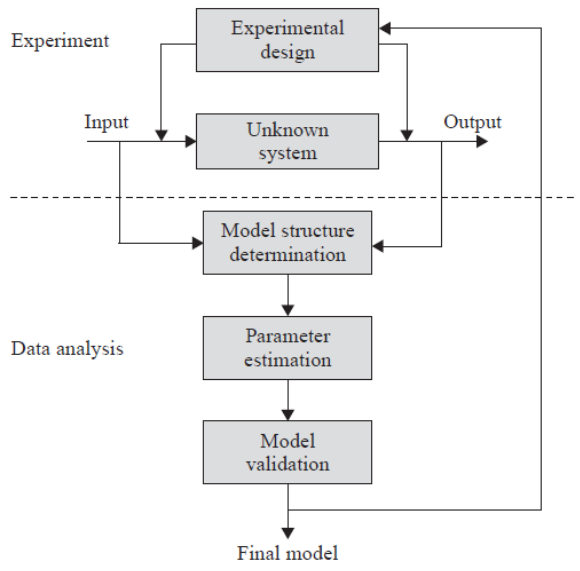
\includegraphics[width=0.5\linewidth]{immagini/validazionedelmodello.png}
\end{figure}

\newpage
\section{Soluzione e Simulazione}

L'ultimo passo della modellizzazione prevede la \textbf{soluzione} delle equazioni. Quando possibile, si ricercano soluzioni analitiche in forma chiusa, ma più frequentemente — a causa delle non-linearità e dell'elevato numero di variabili — è necessario ricorrere a metodi di ottimizzazione e integrazione numerica tramite computer.

Una volta risolto e validato, il modello diviene un simulatore a tutti gli effetti. La \textbf{simulazione} fornisce informazioni preziose, permette di prevedere comportamenti inesplorati e può portare a nuove scoperte. Soprattutto, la simulazione al calcolatore costituisce un'alternativa irrinunciabile all'esperimento sul sistema reale ogniqualvolta quest'ultimo risulti inaccessibile, pericoloso per il paziente, eticamente scorretto, eccessivamente costoso o temporalmente impraticabile.
%\chapter{Modelli di Dati}
I \textbf{modelli dei dati} (noti anche come modelli \textit{data-driven} o \textit{black-box}) forniscono una descrizione quantitativa di un sistema biologico attraverso l'analisi diretta dei dati sperimentali di ingresso e di uscita (input/output). A differenza dei modelli a base fisiologica (white-box), in questo approccio vi \`e solo una corrispondenza implicita tra il modello matematico impiegato e la reale fisiologia del sistema che dà luogo alle misure. Il sistema stesso viene spesso trattato come un blocco (es. un sistema Lineare Tempo-Invariante, o LTI) di cui si analizzano le risposte $y(t)$ a determinati stimoli $x(t)$.

\section{Quando utilizzare un modello dei dati?}
L'impiego di un approccio \textit{black-box} \`e particolarmente indicato nelle seguenti condizioni:
\begin{enumerate}
    \item Non si ha a disposizione una conoscenza approfondita o completa della fisiologia del sistema. Questa condizione \`e tipica, ad esempio, in ambiti complessi come l'elettrofisiologia e la neurofisiologia.
    \item Una semplice rappresentazione della relazione input/output del sistema \`e sufficiente per gli scopi della ricerca o dell'applicazione clinica.
    \item Non sussiste la necessità di specificare e modellare i meccanismi fisiologici fondamentali alla base del comportamento del sistema.
\end{enumerate}

\section{Categorie di Approccio ai Modelli dei Dati}
L'applicazione dei modelli dei dati in fisiologia e medicina pu\`o essere classificata in cinque categorie principali, a seconda del tipo di variabili misurate e dello scopo della modellizzazione.

\subsection{1. Variabile singola ottenuta spontaneamente}
Questa categoria analizza i ritmi e le oscillazioni biologiche naturali senza l'applicazione di perturbazioni esterne.
\begin{itemize}
    \item \textbf{Temperatura corporea:} Un classico esempio \`e la variazione del ritmo biologico della temperatura corporea durante il ciclo mestruale femminile, caratterizzato da una periodicità mensile. In prima approssimazione, questo andamento pu\`o essere descritto in modo efficace mediante una funzione sinusoidale:
    \begin{equation}
        y = A_1 \sin\left[ \frac{6.2832(A_2 + t)}{A_3} \right] + A_4
    \end{equation}
    dove i parametri stimati dai dati rappresentano l'ampiezza dell'oscillazione ($A_1 \approx 0.191 ^\circ\text{C}$), lo sfasamento ($A_2 \approx 12.85 \text{ giorni}$), il periodo ($A_3 \approx 27.07 \text{ giorni}$) e il valore medio ($A_4 \approx 36.56 ^\circ\text{C}$).
    
    \item \textbf{Ritmi gastro-intestinali:} I dati elettrici del tratto gastro-intestinale possono essere modellizzati impiegando complessi sistemi di oscillatori non lineari. Ad esempio, l'attività può essere riprodotta mediante un \textit{oscillatore di Van der Pol}:
    \begin{equation}
        \frac{d^2x}{dt^2} - \epsilon(\alpha^2 - x^2)\frac{dx}{dt} + \omega^2 x = 0
    \end{equation}
    I parametri da determinare dai dati sono $\epsilon$, $\alpha$ e $\omega$, i quali definiscono rispettivamente la forma, l'ampiezza e la frequenza dell'oscillazione. Per modellizzare l'intero intestino umano (lungo circa 240 cm), \`e necessario concatenare una rete di circa 100 oscillatori di questo tipo accoppiati tra loro.
\end{itemize}

\subsection{2. Variabile singola in risposta ad una perturbazione}
In questo caso, si analizza la variazione di una singola grandezza fisiologica a seguito di un evento controllato, come una \textbf{terapia farmacologica}.
Un esempio applicativo \`e la predizione della risposta polmonare in pazienti affetti da disturbo cronico ostruttivo (COPD) a seguito della somministrazione di un broncodilatatore (la teofillina). Il modello permette di aggiustare il dosaggio ottimale valutando l'effetto terapeutico:
\begin{equation}
    FVC = m C_{p_{ss}} + i
\end{equation}
dove \textit{FVC} (Forced Vital Capacity) rappresenta la risposta ventilatoria (capacità vitale forzata), $C_{p_{ss}}$ \`e la concentrazione \textit{steady-state} del farmaco nel plasma, $m$ \`e la sensibilità individuale al farmaco, e $i$ \`e il livello di base di FVC in assenza di trattamento.

\subsection{3. Due variabili legate causalmente}
Nello studio dei sistemi endocrini e metabolici, \`e frequente dover descrivere la relazione \textbf{ormone/ormone} (es. Testosterone/LH) oppure \textbf{substrato/ormone} (es. Glucosio/C-peptide). Storicamente, per analizzare la sincronia di secrezione, si sono utilizzati metodi classici come la \textit{cross-correlazione} e l'analisi dei \textit{cross-spettri}. Tuttavia, questi metodi matematici si rivelano poco performanti quando si dispone di una scarsa quantità di dati o in presenza di misure altamente rumorose. Una valida alternativa utilizzata nella modellistica odierna \`e lo studio della \textit{coerenza dei picchi} di secrezione.

\subsection{4. Modelli input-output per il controllo}
Questi modelli sono tipici dei sistemi fisiologici di regolazione (omeostasi), rappresentabili mediante schemi a blocchi e sistemi controreazionati (feedback).
\begin{itemize}
    \item \textbf{Controllo della pupilla:} La quantità di luce che entra nella retina ($L_c$) \`e determinata dal diametro della pupilla. Se la luce in ingresso supera un valore di riferimento ($L_{REF}$), il riflesso pupillare contrae l'iride riducendo la radiazione. Questo sistema di controllo controreazionato pu\`o essere studiato nel dominio della frequenza (risposta \textit{open-loop}). La funzione di trasferimento $G(s)$ derivata empiricamente dai dati di ampiezza e fase mostra la forma:
    \begin{equation}
        G(s) = \frac{0.16 \exp(-0.18s)}{(1 + 0.1s)^3}
    \end{equation}
    con un guadagno stimato pari a $0.16$.
    
    \item \textbf{Regolazione del glucosio:} In condizioni di salute, l'insulina secreta dal pancreas regola il glucosio. Nei soggetti con diabete di tipo 1, le cellule beta pancreatiche perdono la loro funzione. Il sistema di controllo fisiologico viene meno e deve essere sostituito da un "controllore esterno" (infusione di insulina esogena), concetto alla base dello sviluppo del \textit{pancreas artificiale}.
\end{itemize}

\subsection{5. Modelli input-output: Deconvoluzione}
La stima della risposta impulsiva \`e fondamentale per caratterizzare compiutamente un sistema lineare. Considerando un sistema LTI, l'uscita $c(t)$ in base all'ingresso $u(t)$ \`e data dall'\textbf{integrale di convoluzione}:
\begin{equation}
    c(t) = \int_{-\infty}^{t} g(t-\tau)u(\tau)d\tau
\end{equation}
dove $g(t)$ \`e la risposta impulsiva del sistema (l'uscita a fronte di un ingresso a delta di Dirac $\delta(t)$).
\\
L'uso dell'integrale di convoluzione si distingue in due branche:
\begin{enumerate}
    \item \textbf{Problema Diretto:} Conoscendo l'input (es. dosaggio di un farmaco) e la risposta impulsiva del sistema, si stima l'uscita (es. livello terapeutico e concentrazione nel tempo).
    \item \textbf{Problema Inverso (Deconvoluzione):} Modalità ben più potente in ambito fisiologico. Conoscendo la risposta impulsiva e misurando l'uscita, si stima un \textit{ingresso non direttamente misurabile in vivo} (es. il tasso di secrezione di una ghiandola).
\end{enumerate}

\subsubsection*{Esempio clinico di Deconvoluzione: Secrezione di Insulina}
Per stimare il tasso di secrezione dell'insulina da parte del pancreas, si misurano i dati di concentrazione plasmatica del \textbf{C-peptide} (un sottoprodotto della sintesi dell'insulina).
Si calcola innanzitutto la risposta impulsiva $g(t)$ del C-peptide somministrando un bolo ed effettuando campionamenti frequenti (la curva \`e approssimata tipicamente come somma di due esponenziali). Successivamente, misurando la concentrazione plasmatica nel tempo e applicando l'operazione matematica di \textbf{deconvoluzione}, si pu\`o ricostruire con precisione l'andamento pulsatile (ultradiano) del tasso di secrezione endogena di insulina ($u(t)$ espresso in pmol/min), sia in condizioni basali che durante un test endovenoso di tolleranza al glucosio (IVGTT).
\chapter{Identificazione dei modelli}
L'identificazione di un modello matematico per un sistema biologico richiede un'attenta transizione dal sistema reale alla sua rappresentazione formale. Questo processo si articola tipicamente in due passaggi fondamentali: in primo luogo, è necessario definire la struttura matematica del modello (determinazione della struttura); in secondo luogo, occorre determinare quantitativamente tutti i parametri associati a tale struttura. Quest'ultima fase, che prende il nome di \textbf{identificazione}, unita al primo passo, fornisce il modello matematico nella sua forma completa.

\section{Raccolta Dati e Disegno Sperimentale}
Per poter risolvere il problema dell'identificazione e stimare i parametri del modello, il prerequisito fondamentale è la \textbf{disponibilità di dati}. In alcuni casi, i dati possono provenire dalle dinamiche intrinseche del sistema biologico stesso, come oscillazioni spontanee o rumore fisiologico di fondo. Tuttavia, più frequentemente è necessario intervenire in modo attivo definendo un apposito disegno sperimentale (\emph{experimental design}) finalizzato alla raccolta mirata dei dati. Un esperimento tipico consiste nell'applicare al sistema in esame specifici segnali di test (variabili di input) e registrarne l'evoluzione temporale della risposta (variabili di output).

\section{Selezione dei Segnali di Test}
La scelta dei segnali di eccitazione non è arbitraria, ma è guidata da specifici criteri tesi a massimizzare le informazioni raccolte preservando la natura del sistema:
\begin{itemize}
    \item \textbf{Fattibilità e adeguatezza:} I segnali di test devono essere convenienti da generare e adatti al sistema in esame. Esempi classici includono la somministrazione di un farmaco mediante iniezione in bolo per gli studi di farmacocinetica, o una variazione a gradino nella concentrazione di ossigeno inalato per studiare la dinamica del sistema respiratorio.
    \item \textbf{Ampiezza e vincoli di sicurezza:} I segnali devono essere il più ampi possibile al fine di produrre un output caratterizzato da un elevato rapporto segnale/rumore. Tuttavia, si scontrano con vincoli pratici inderogabili: occorre rispettare severe considerazioni etiche e di sicurezza sulla salute del paziente o del campione biologico. Inoltre, da un punto di vista sistemistico, il disturbo introdotto non deve allontanare il sistema dalla regione di linearità in cui il modello strutturale risulta valido.
    \item \textbf{Efficienza temporale:} Il segnale di test ideale deve minimizzare il tempo complessivo necessario allo svolgimento dell'esperimento e al successivo processo di identificazione.
\end{itemize}

In generale, i segnali di test impiegati nella pratica sperimentale si classificano in tre grandi categorie: segnali che producono una risposta transitoria, segnali che producono una risposta in frequenza (armonici) e segnali casuali.

\subsection{Segnali Transitori}
I segnali di test che producono una risposta transitoria sono quelli maggiormente impiegati, specialmente in ambiti come gli studi metabolici e la farmacocinetica. Le forme di input più usuali sono l'impulso (iniezione) e il gradino (un'infusione continua o variazione a gradino di gas). Una volta applicato l'ingresso, si osserva la risposta impulsiva o la risposta a gradino del sistema, che sono matematicamente legate tra loro.
\begin{figure}[h]
    \centering
    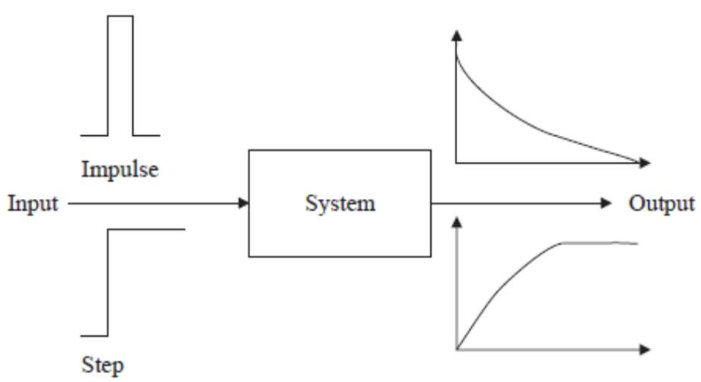
\includegraphics[width=0.5\linewidth]{immagini/segnali_di_test_transitori.png}
\end{figure}

Il test della risposta impulsiva presenta il vantaggio di essere proceduralmente semplice e di breve durata, in quanto l'interesse risiede unicamente nel comportamento transitorio e non nell'analisi delle dinamiche a regime. Ciononostante, presenta dei limiti pratici nell'applicazione:
\begin{enumerate}
    \item L'ampiezza dell'impulso rappresenta un compromesso delicato: se il segnale è troppo piccolo, provoca un'inadeguata eccitazione del sistema; se è eccessivamente grande, rischia di portare il sistema fuori dalla sua regione di validità lineare.
    \item Non vi è alcun filtraggio intrinseco del rumore; questo comporta che rumore ambientale o altri input non controllati possano generare un elevato errore sull'uscita registrata.
    \item Nelle applicazioni in vivo, vi è un numero ristretto di siti anatomici per la somministrazione e la frequenza di campionamento tramite prelievi è limitata, portando talvolta all'uso di tecniche di imaging come alternativa meno invasiva.
\end{enumerate}

\subsection{Segnali Armonici}
Il test della risposta in frequenza consiste nell'applicare segnali armonici (sinusoidi pure) a diverse frequenze e osservare gli effetti che il sistema produce sull'uscita, misurandone l'amplificazione (o attenuazione) e lo sfasamento. Se si considera un sistema lineare tempo-invariante (LTI), applicando in ingresso un segnale $A \sin(\omega t)$, l'uscita a regime sarà data da:
\[
y(t) = A |G(j\omega)| \sin(\omega t + \angle G(j\omega))
\]
dove $G(j\omega)$ è la funzione di trasferimento in frequenza del sistema.
\begin{figure}
    \centering
    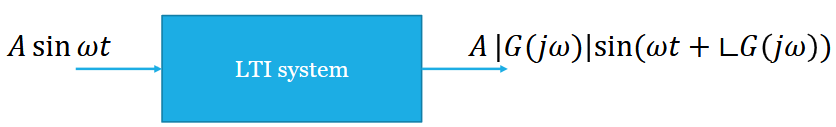
\includegraphics[width=0.7\linewidth]{immagini/segnali di test armonici.png}
\end{figure}
Pur essendo meno convenienti da applicare da un punto di vista pratico e richiedendo spesso strumentazione speciale (come analizzatori di spettro), i segnali armonici presentano notevoli vantaggi. Consentono di eccitare selettivamente tutti i modi del sistema senza dover somministrare segnali di ampiezza eccessiva. Garantiscono inoltre un ottimo filtraggio intrinseco del rumore, poiché l'analisi dell'uscita si concentra su una sola componente in frequenza alla volta. Un notevole svantaggio risiede nella lunga durata del test: ogni frequenza va testata singolarmente, ed è necessario un tempo di attesa sufficiente per far decadere gli effetti transitori iniziali in modo da misurare unicamente la componente a regime. I dati di risposta in frequenza raccolti possono poi essere impiegati per adattare (fittare) modelli parametrici al fine di stimare i parametri incogniti del sistema.

\subsection{Segnali Random}
I segnali random offrono una terza via molto interessante per l'identificazione. Consideriamo un sistema LTI con risposta impulsiva $g(t)$. Applicando in ingresso un segnale generico $m(t)$ e misurando l'uscita $y(t)$, si può dimostrare che la funzione di cross-correlazione tra l'ingresso e l'uscita, indicata con $R_{my}(\tau)$, è legata all'autocorrelazione dell'ingresso $R_{mm}$ e alla risposta impulsiva dalla seguente equazione integrale di convoluzione:
\[
R_{my}(\tau) = \int_{-\infty}^{\infty} g(t) R_{mm}(t-\tau) d\tau = g*R_{mm}
\]
Se come input si sceglie un segnale che approssima il \textbf{rumore bianco} (caratterizzato da uno spettro con densità di potenza costante a tutte le frequenze e da un'autocorrelazione impulsiva), la relazione si semplifica notevolmente, restituendo direttamente:
\[
R_{my}(\tau) = g(\tau)
\]
Il test prevede quindi l'applicazione di un segnale di tipo rumore bianco (nella pratica, spesso si usano sequenze binarie pseudo-random o PRBS) calcolando poi a posteriori la cross-correlazione per ricostruire la risposta impulsiva $g(t)$. 
Poiché un segnale casuale eccita lo spettro su tutte le frequenze, questo test equivale a eseguire test armonici multipli contemporaneamente, rendendolo concettualmente più rapido, seppur più oneroso sul piano computazionale. Il processo di integrazione necessario al calcolo della cross-correlazione funge da eccellente filtro per le componenti di rumore estranee. Va notato che, per assicurare l'accuratezza statistica della stima della cross-correlazione, il test deve comunque essere protratto per un intervallo di tempo sufficientemente lungo.
\newpage
\section{Sorgenti di Errore}
L'operazione di stima dei parametri è fisiologicamente affetta da diverse sorgenti di errore e rumore, inquadrabili nelle seguenti categorie:

\begin{wrapfigure}{r}{0.5\textwidth}
  \begin{center}
    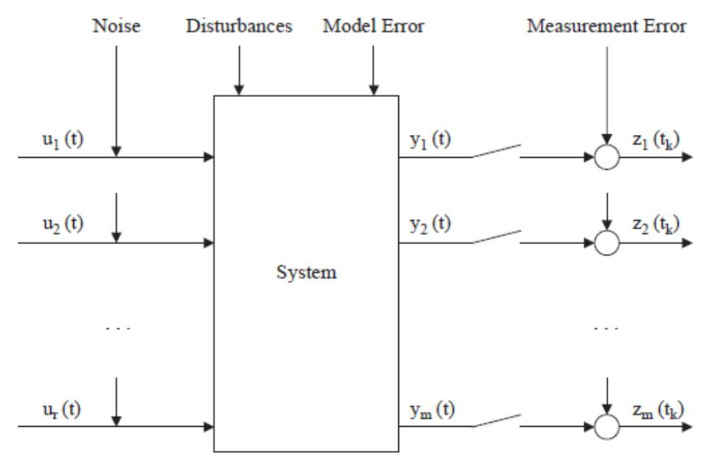
\includegraphics[width=0.5\textwidth]{immagini/sorgenti di errore.png}
  \end{center}
\end{wrapfigure}
\begin{itemize}
    \item \textbf{Imperfezioni del segnale di test:} L'input reale spesso si discosta dalla forma teorica ideale assunta matematicamente (ad esempio, un impulso non infinitamente stretto o un segnale random che non è un vero rumore bianco).
    \item \textbf{Errori di misura:} Rappresentano l'incertezza e il rumore della strumentazione sulle misurazioni delle variabili di uscita. 
    \item \textbf{Disturbi:} Fluttuazioni e interferenze da parte di altre variabili esterne al sistema.
    \item \textbf{Errore di modello:} Discrepanza sistematica tra la struttura formale postulata (la matematica) e la realtà del processo biologico sottostante.
\end{itemize}

Tra questi, l'\textbf{errore di misura} è l'unico che può essere modellato e trattato in maniera analiticamente rigorosa. Tradizionalmente, si assume un'ipotesi di additività dell'errore. Denotando con $z_l$ la misura campionata all'istante $t_i$, con $y_l$ l'uscita predetta dal modello per un dato vettore di parametri $p$, e con $v_l$ il termine di errore aleatorio, possiamo scrivere:
\begin{equation}
\begin{split}
    z_l(t_i, p) &= y_l(t_i, p) + v_l(t_i) \\ \text{per } i&=1,2,\dots,N_l \\ e \quad l&=1,2,\dots,m
\end{split}
\end{equation}
Per consentire algoritmi di identificazione robusti, è necessario fornire una caratterizzazione statistica adeguata di $v_l$ (ad esempio, ipotizzando una distribuzione gaussiana o poissoniana, rumore bianco, o scorrelato nel tempo). Quanto più precisa sarà questa caratterizzazione teorica, tanto minore sarà l'impatto negativo dell'errore sull'affidabilità della stima dei parametri. Se non avessimo errori di misura le nostre misure sarebbero deterministiche. 
\newpage
\section{Il Processo di Identificazione}
A livello concettuale, il problema complessivo dell'identificazione si biforca spesso in due tipologie distinte di analisi: la stima dei parametri e la stima dei segnali.

\subsection{Stima dei Parametri}
Prima di lanciare algoritmi per la stima numerica, occorre necessariamente verificare l'\textbf{identificabilità a priori} del modello. Questa analisi teorica risponde a una domanda fondamentale: indipendentemente dall'errore nei dati, ho misurato un numero sufficiente di variabili per poter stimare in maniera univoca tutti i parametri interni del modello strutturale? 

Nel caso in cui l'identificabilità non sia garantita (ad esempio, la stima risulta non univoca), si presentano due soluzioni pratiche:
\begin{enumerate}
    \item Ridurre la complessità e l'ordine del modello, abbassando il numero di parametri da stimare, avendo cura di validare se la versione semplificata rimane adeguata al contesto fisiologico.
    \item Aumentare la base di dati, aggiungendo un nuovo esperimento o iniziando a misurare un'ulteriore variabile di output precedentemente non osservata.
\end{enumerate}
Una volta che il sistema risulti a priori identificabile, si procede alla stima. Tra le tecniche più consolidate figurano gli approcci ai minimi quadrati (sia lineari che non lineari), i metodi basati sul principio della massima verosimiglianza (\emph{Maximum Likelihood}), e l'approccio probabilistico Bayesiano.

\subsection{Stima del Segnale}
Non sempre l'obiettivo è ricavare i parametri numerici (resistenza, costante di decadimento, ecc.) del sistema biologico. A volte, si intende stimare l'andamento di un segnale incognito. Tipicamente le relazioni analizzate mettono in gioco tre grandezze: il segnale di input, la risposta impulsiva del sistema, e il segnale di output misurato. 
Quando ne conosciamo due e vogliamo stimare la terza, applichiamo algoritmi focalizzati sui segnali (come ad esempio la \emph{deconvoluzione}, necessaria quando si intende risalire all'input originario conoscendo il sistema e l'uscita). Per gestire l'intrinseca instabilità di tali calcoli, si fa spesso ricorso a tecniche matematiche avanzate note come algoritmi di \emph{regolarizzazione}.
%input{Capitoli/999-Richiami_di_elettrofisiologia}
\appendix
\chapter{Domande delle lezioni}
\begin{enumerate}
    \item 
\end{enumerate}

\end{document}
